\documentclass[cjk,slidestop,compress,mathserif,blue]{beamer}
%dvipdfm选项是关键,否则编译统统通不过
%beamer的颜色选项定义的是导航条和标题的颜色(即关键词structure的颜色)

%%%%%%%%%%%%%%%%仅限于XeTeX可使用的宏包%%%%%%%%%%%%%%%%%%%%%%%%%%%%
\usepackage{fontspec,xunicode,xltxtra,beamerthemesplit}
%\usepackage{beamerthemesplit}
\usepackage{handoutWithNotes}		%(讲义)在打印PPT的时候会留出给每一页做注释的部分
\usepackage{xeCJK}
\setCJKmainfont[BoldFont=黑体, ItalicFont=楷体, BoldItalicFont=仿宋]{黑体}
%\setsansfont[Mapping=tex-text]{Adobe 黑体 Std}
%如果装了Adobe Acrobat,可在font.conf中配置Adobe字体的路径以使用其中文字体
%也可直接使用系统中的中文字体如SimSun,SimHei,微软雅黑 等
%原来beamer用的字体是sans family;注意Mapping的大小写,不能写错

\usepackage{listings} 
\lstset{language=Matlab}%代码语言使用的是matlab 
\lstset{breaklines}%自动将长的代码行换行排版 
\lstset{extendedchars=false}%解决代码跨页时,章节标\dots

%%%%%%%%   确定标题和导航条结构的框架     %%%%%%%%%%%%
\usepackage{beamerthemeshadow}                       %
%\usepackage{beamerthemeclassic}%导航条色与背景色一致%
%\usepackage{authblk}				     %作者地址和E-mail
%%%%%%%%%%%%%%%%%%%%%%%%%%%%%%%%%%%%%%%%%%%%%%%%%%%%%%
\setbeamerfont{roman title}{size={}}
%\usepackage{CJK} % CJK 中文支持                                  %
\usepackage{amsmath,amsthm,amsfonts,amssymb,bm}
\usepackage{bbding}
\usepackage{mathrsfs}
\usepackage{xcolor}                                        %使用默认允许使用颜色
\usepackage{hyperref} 
\usepackage{graphicx}
\usepackage{subfigure}           %图片跨页
\usepackage{animate}		 %插入动画
\usepackage{tikz}		 %绘图工具
\usepackage{caption}
\captionsetup{font=footnotesize}

%\usepackage[version=3]{mhchem}		%化学公式
\usepackage{chemformula}
\usepackage{chemfig}		%化学公式

\usepackage{multirow}
\usepackage{makecell}		%允许单元格内换行

\usepackage[dvipdfmx]{movie15_dvipdfmx} %插入视频
%\usepackage{handoutWithNotes}		%(讲义)在打印PPT的时候会留出给每一页做注释的部分
%\pgfpagesuselayout{1 on 1 with notes landscape}[a4paper,border shrink=5mm]

%%%%%%%%%%%%%%%%%%%%%%BIBTEX 引用参考文献%%%%%%%%%%%%%%%%%%%%%%%%%%%%%%%%%%%%%%%%%%%%%%%%
%\usepackage{filecontents}
%\begin{filecontents*}{main.bib}
%@techreport{2012FracfocusChemical,
%  author = {FracFocus,},
%  howpublished = {\url{http://fracfocus.org/water-protection/drilling-usage}},
%  institution = {The Ground Water Protection Council and Interstate Oil and Gas
%  Compact Commission},
%  month = {feb},
%  title = {{Chemical Use In Hydraulic Fracturing}},
%  year = {2012}
%}
%\end{filecontents*}
%\usepackage[backend=bibtex,sorting=none]{biblatex}
%%\usepackage[backend=biber,style=authoryear]{biblatex}
%\addbibresource{main.bib} %BibTeX数据文件及位置

%\usepackage[numbers,sort&compress]{natbib} %紧密排列             %
\usepackage[sectionbib]{chapterbib}        %每章节单独参考文献   %
\usepackage{hypernat}                                                                         %
\setbeamertemplate{bibliography item}[text] %参考文献前标注[]
%\usepackage[dvipdfm,bookmarksopen=true,pdfstartview=FitH,CJKbookmarks]{hyperref}		%
\hypersetup{bookmarksnumbered,colorlinks,linkcolor=brown,citecolor=blue,urlcolor=red}         %
%参考文献含有超链接引用时需要下列宏包,注意与natbib有冲突        %
%\usepackage[dvipdfm]{hyperref}                                  %
%\usepackage{hypernat}                                           %
\newcommand{\upcite}[1]{\hspace{0ex}\textsuperscript{\cite{#1}}} %

%\usepackage{marvosym} %插入各种符号

%\useoutertheme{smoothbars}
\useinnertheme[shadow=true]{rounded}
\usetheme{Berkeley}                                          %主题式样
%\usetheme{Luebeck}

\usecolortheme{lily}                                        %颜色主题式样

\usefonttheme{professionalfonts}                           %字体主题样式宏包

%\beamertemplatetransparentcoveredhigh                      %使所有被隐藏的文本高度透明
\beamertemplatetransparentcovereddynamicmedium             %使所有被隐藏的文本完全透明,动态,动态的范围很小
\mode<presentation>
%\beamersetaveragebackground{gray}                          %设置背景颜色(单一色) 
\beamertemplateshadingbackground{green!10}{red!5}         %设置背景颜色(渐变色)

%i放置单位logo
%\logo{
\includegraphics[width=1.6cm,height=0.35cm]{Figures/BCC_logo-1.png}}	%简单设置logo

%\pgfdeclareimage[width=3.5cm]{logoname}{Figures/BCC_logo-1.png}		%logo置于左侧微调
%\logo{\pgfuseimage{logoname}{\vspace{0.2cm}\hspace*{-2.0cm}}}

%在指定位置精确放置logo
%\usepackage{tikz}
\usepackage{beamerfoils}
\usepackage{pgf}
\logo{\pgfputat{\pgfxy(10.68,0.00)}{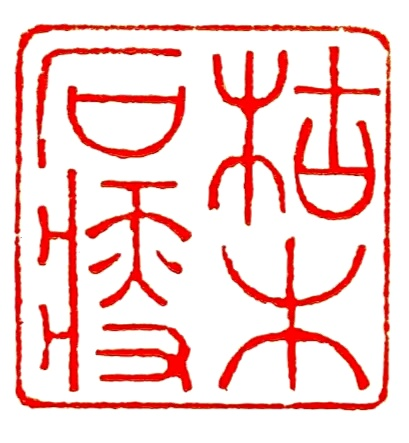
\includegraphics[height=1.20cm,viewport=0 15 400 430,clip]{Figures/seal_Jiang-2.jpg}}
      %\pgfputat{\pgfxy(10.817,-0.218)}{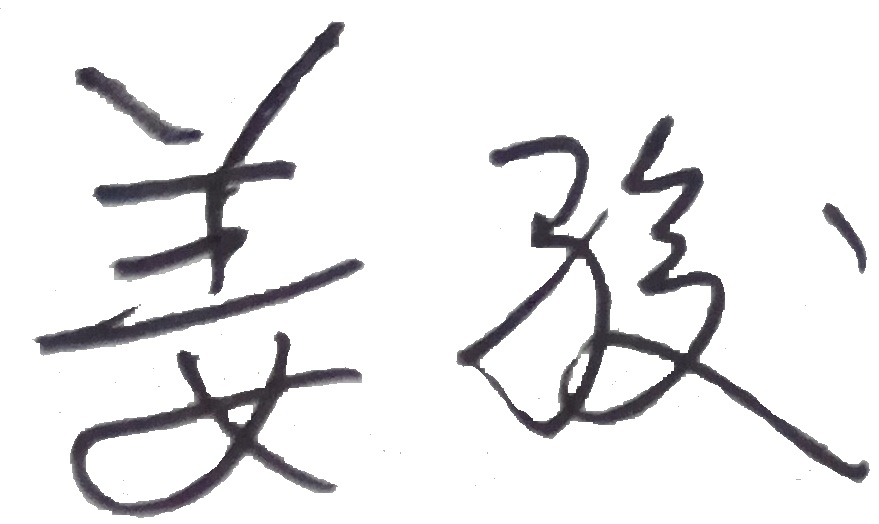
\includegraphics[height=0.47cm,viewport=20 0 670 350,clip]{Figures/signature_Jiang_new.jpg}}
}
%\logo{\pgfputat{\pgfxy(11.68,0.252)}{
\includegraphics[height=0.89cm,viewport=0 15 810 800,clip]{Figures/seal_Jiang-new.jpg}}\pgfputat{\pgfxy(10.762,-0.218)}{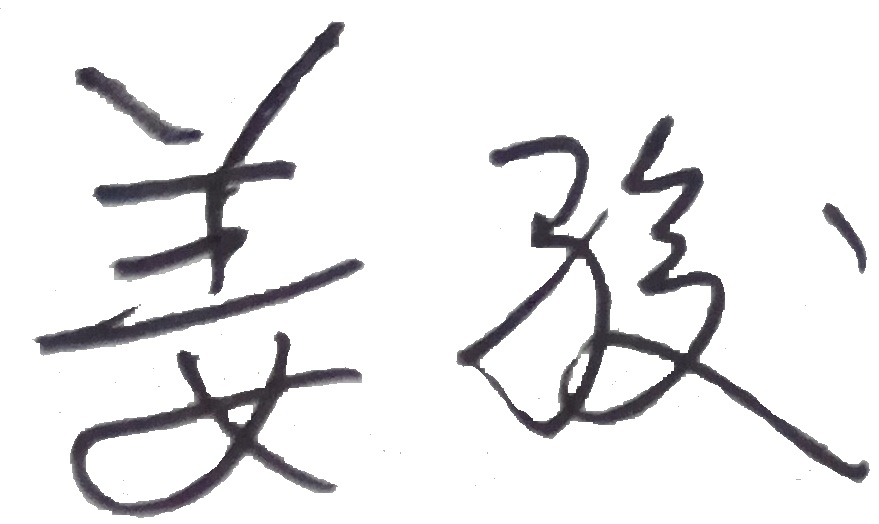
\includegraphics[height=0.49cm,viewport=20 0 670 350,clip]{Figures/signature_Jiang_new.jpg}}}
%\logo{\pgfputat{\pgfxy(11.68,0.252)}{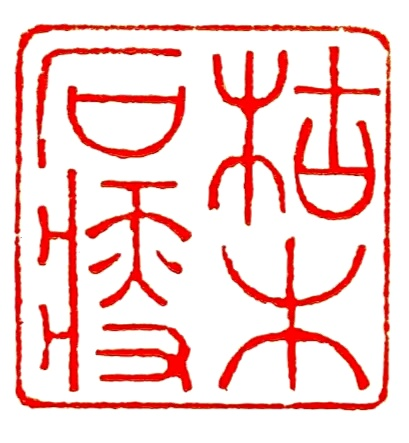
\includegraphics[height=0.90cm,viewport=0 15 400 430,clip]{Figures/seal_Jiang-2.jpg}}\pgfputat{\pgfxy(10.817,-0.218)}{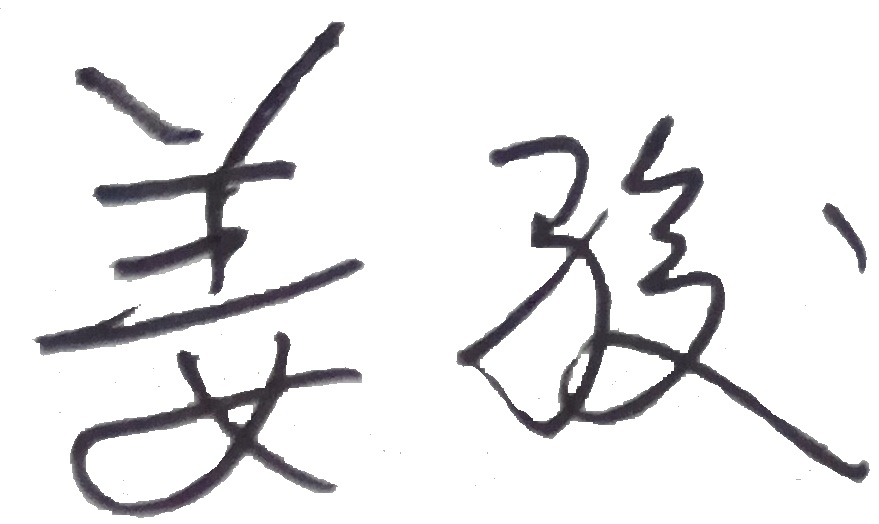
\includegraphics[height=0.47cm,viewport=20 0 670 350,clip]{Figures/signature_Jiang_new.jpg}}}
%\logo{\pgfputat{\pgfxy(11.68,0.15)}{
\includegraphics[height=1.01cm,viewport=0 0 140 120,clip]{Figures/BCC_logo-1.png}}\pgfputat{\pgfxy(10.502,-0.218)}{
\includegraphics[height=0.369cm,viewport=140 0 540 120,clip]{Figures/BCC_logo-1.png}}}
%\logo{\pgfputat{\pgfxy(11.68,0.15)}{
\includegraphics[height=0.95cm,viewport=0 0 510 360,clip]{Figures/Logo_Gainstrong.png}}\pgfputat{\pgfxy(10.333,-0.195)}{
\includegraphics[height=0.35cm,viewport=530 70 1100 218,clip]{Figures/Logo_Gainstrong.png}}}
%\logo{\pgfputat{\pgfxy(10.28,0.00)}{
\includegraphics[height=0.95cm,viewport=0 0 1100 360,clip]{Figures/Logo_Gainstrong.png}}}
%\logo{\pgfputat{\pgfxy(11.68,0.15)}{
\includegraphics[height=0.95cm,viewport=0 0 510 360,clip]{Figures/Logo_Gainstrong.png}}\pgfputat{\pgfxy(10.333,-0.195)}{
\includegraphics[height=0.35cm,viewport=530 70 1100 218,clip]{Figures/Logo_Gainstrong.png}}}
%\MyLogo{
%	\pgfputat{\pgfxy(-50,-50)}{\pgfbox[right,base]{
\includegraphics[height=1cm]{Figures/BCC_logo-1.png}}}

%logo作为背景放置
%\setbeamertemplate{background}{
%	\pgfputat{\pgfxy(6.5,-0.5)}{\pgfbox[left,top]{\pgfimage[height=1.1cm]{Figures/BCC_logo-1.png}}}}

%\logo{}									%不显示logo

\begin{document}
%\begin{CJK*}{GBK}{song}
%\begin{CJK*}{GBK}{kai}
%beamer下不能用\songyi、\zihao等命令!
%\graphicspath{Figures/}

%\renewcommand{\figurename}{\tiny\CJKfamily{hei} 图.}
\renewcommand{\figurename}{\tiny{\bf Fig}.}
%\renewcommand{\tablename}{\tiny\CJKfamily{hei} 表.}
\renewcommand{\tablename}{\tiny{\bf Tab}.}
%\renewcommand{\tablename}{\tiny\CJKfamily{hei} 表.}
%\renewcommand{\thesubfigure}{\roman{subfigure}}  %\makeatletter 子图标记罗马字母
\renewcommand{\thesubfigure}{\tiny(\alph{subfigure})}  %\makeatletter 子图标记英文字母
%\renewcommand{\thesubfigure}{}  \makeatletter %子图无标记

%%%%%%%%%%%%%%%%%%%%%%%%%%%%%%% Latex 的 tikz 绘图 %%%%%%%%%%%%%%%%%%%%%%%%%%%%%%%%%%%%%%%%%%%
%\begin{tikzpicture}
%    % 引入图片
%    \node[anchor=south west,inner sep=0] (image) at (0,0) {\includegraphics[width=0.9\textwidth]{Mycena_interrupta.jpg}};
%
%    \begin{scope}[x={(image.south east)},y={(image.north west)}]
%        % 建立相对坐标系
%        \draw[help lines,xstep=.1,ystep=.1] (0,0) grid (1,1);
%        \foreach \x in {0,1,...,9} { \node [anchor=north] at (\x/10,0) {0.\x}; }
%        \foreach \y in {0,1,...,9} { \node [anchor=east] at (0,\y/10) {0.\y}; }
%        % 作图命令
%        \draw[red, ultra thick, rounded corners] (0.62,0.65) rectangle (0.78,0.75);
%    \end{scope}
%\end{tikzpicture}
%%%%%%%%%%%%%%%%%%%%%%%%%%%%%%%%%%%%%%%%%%%%%%%%%%%%%%%%%%%%%%%%%%%%%%%%%%%%%%%%%%%%%%%%%%%%%%

%%%%%%%%%%%%%%%%%%%%%%%%%%%%%%%%%%%%%%%%%%  不使用 authblk 包制作标题  %%%%%%%%%%%%%%%%%%%%%%%%%%%%%%%%%%%%%%%%%%%%%%
%-------------------------------PPT Title-------------------------------------
\title{基于\rm{DFT}的第一原理计算方法简介}
%-----------------------------------------------------------------------------

%----------------------------Author & Date------------------------------------
\author[\textrm{Jun\_Jiang}]{\vskip 20pt 姜\;\;骏\inst{}} %[]{} (optional, use only with lots of authors)
%% - Give the names in the same order as the appear in the paper.
%% - Use the \inst{?} command only if the authors have different
%%   affiliation.
\institute[BCC]{\inst{}%
% \vskip -20pt 北京市计算中心
}
\date[\today] % (optional, should be abbreviation of conference name)
{	{\fontsize{6.2pt}{4.2pt}\selectfont{\textcolor{blue}{E-mail:~}\url{czjiangjun@yeah.net}}}
\vskip 5 pt {\fontsize{8.2pt}{6.2pt}\selectfont{%清华大学\;\;物理系% 报告地点
	\vskip 5 pt \textrm{2021.12}}}
}

%% - Either use conference name or its abbreviation
%% - Not really information to the audience, more for people (including
%%   yourself) who are reading the slides onlin%%   yourself) who are reading the slides onlin%%   yourself) who are reading the slides onlineee
%%%%%%%%%%%%%%%%%%%%%%%%%%%%%%%%%%%%%%%%%%%%%%%%%%%%%%%%%%%%%%%%%%%%%%%%%%%%%%%%%%%%%%%%%%%%%%%%%%%%%%%%%%%%%%%%%%%%%

\subject{}
% This is only inserted into the PDF information catalog. Can be left
% out.
%\maketitle
\frame
{
%	\frametitle{\fontsize{9.5pt}{5.2pt}\selectfont{\textcolor{orange}{“高通量并发式材料计算算法与软件”年度检查}}}
\titlepage
}
%-----------------------------------------------------------------------------

%------------------------------------------------------------------------------列出全文 outline ---------------------------------------------------------------------------------
\section*{}
\frame[allowframebreaks]
{
  \frametitle{Outline}
%  \frametitle{\textcolor{mycolor}{\secname}}
  \tableofcontents%[current,currentsection,currentsubsection]
}
%在每个section之前列出全部Outline
%类似的在每个subsection之前列出全部Outline是\AtBeginSubsection[]
\AtBeginSection[]
{
  \frame<handout:0>%[allowframebreaks]
  {
    \frametitle{Outline}
%全部Outline中,本部分加亮
    \tableofcontents[current,currentsection]
  }
}

%------------------------------------------------------------------------------PPT main Body------------------------------------------------------------------------------------
\small
\section{量子力学基础}
\frame
{
	\frametitle{黑体辐射与能量量子化}
	\textrm{1900}年,为了解释黑体辐射\textrm{(black-body radiation)}的能量密度与辐射频率的关系,\textrm{M.~Planck}引入\textcolor{red}{能量量子化}的假设,利用统计物理推导出与实验符合得非常好的黑体辐射\textrm{Planck~}公式:~
	\begin{displaymath}
		\rho_{\nu}\mathrm{d}{\nu}=\dfrac{8{\pi}h{\nu}^3}{C^3}\bigg(\dfrac1{\mathrm{e}^{h\nu/kT}-1}\bigg)\mathrm{d}\nu
	\end{displaymath}
\begin{figure}[h!]
\centering
\vspace{-10.5pt}
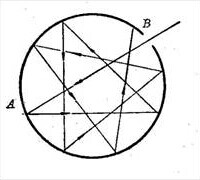
\includegraphics[height=1.45in,width=1.45in,viewport=0 0 136 136,clip]{Figures/Black_box.jpg}
\hskip 1pt
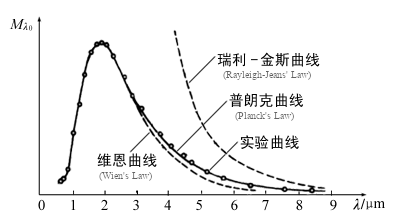
\includegraphics[height=1.32in,width=2.25in,viewport=0 0 390 215,clip]{Figures/Black_box_curve.png}
\caption{\textrm{The black-body radiation and the curve}}
\label{Black_box}
\end{figure}
}

\frame
{
	\frametitle{量子力学的奠基人}
\begin{figure}[h!]
\centering
%\vspace{-25.5pt}
%\hspace*{-15.5pt}
%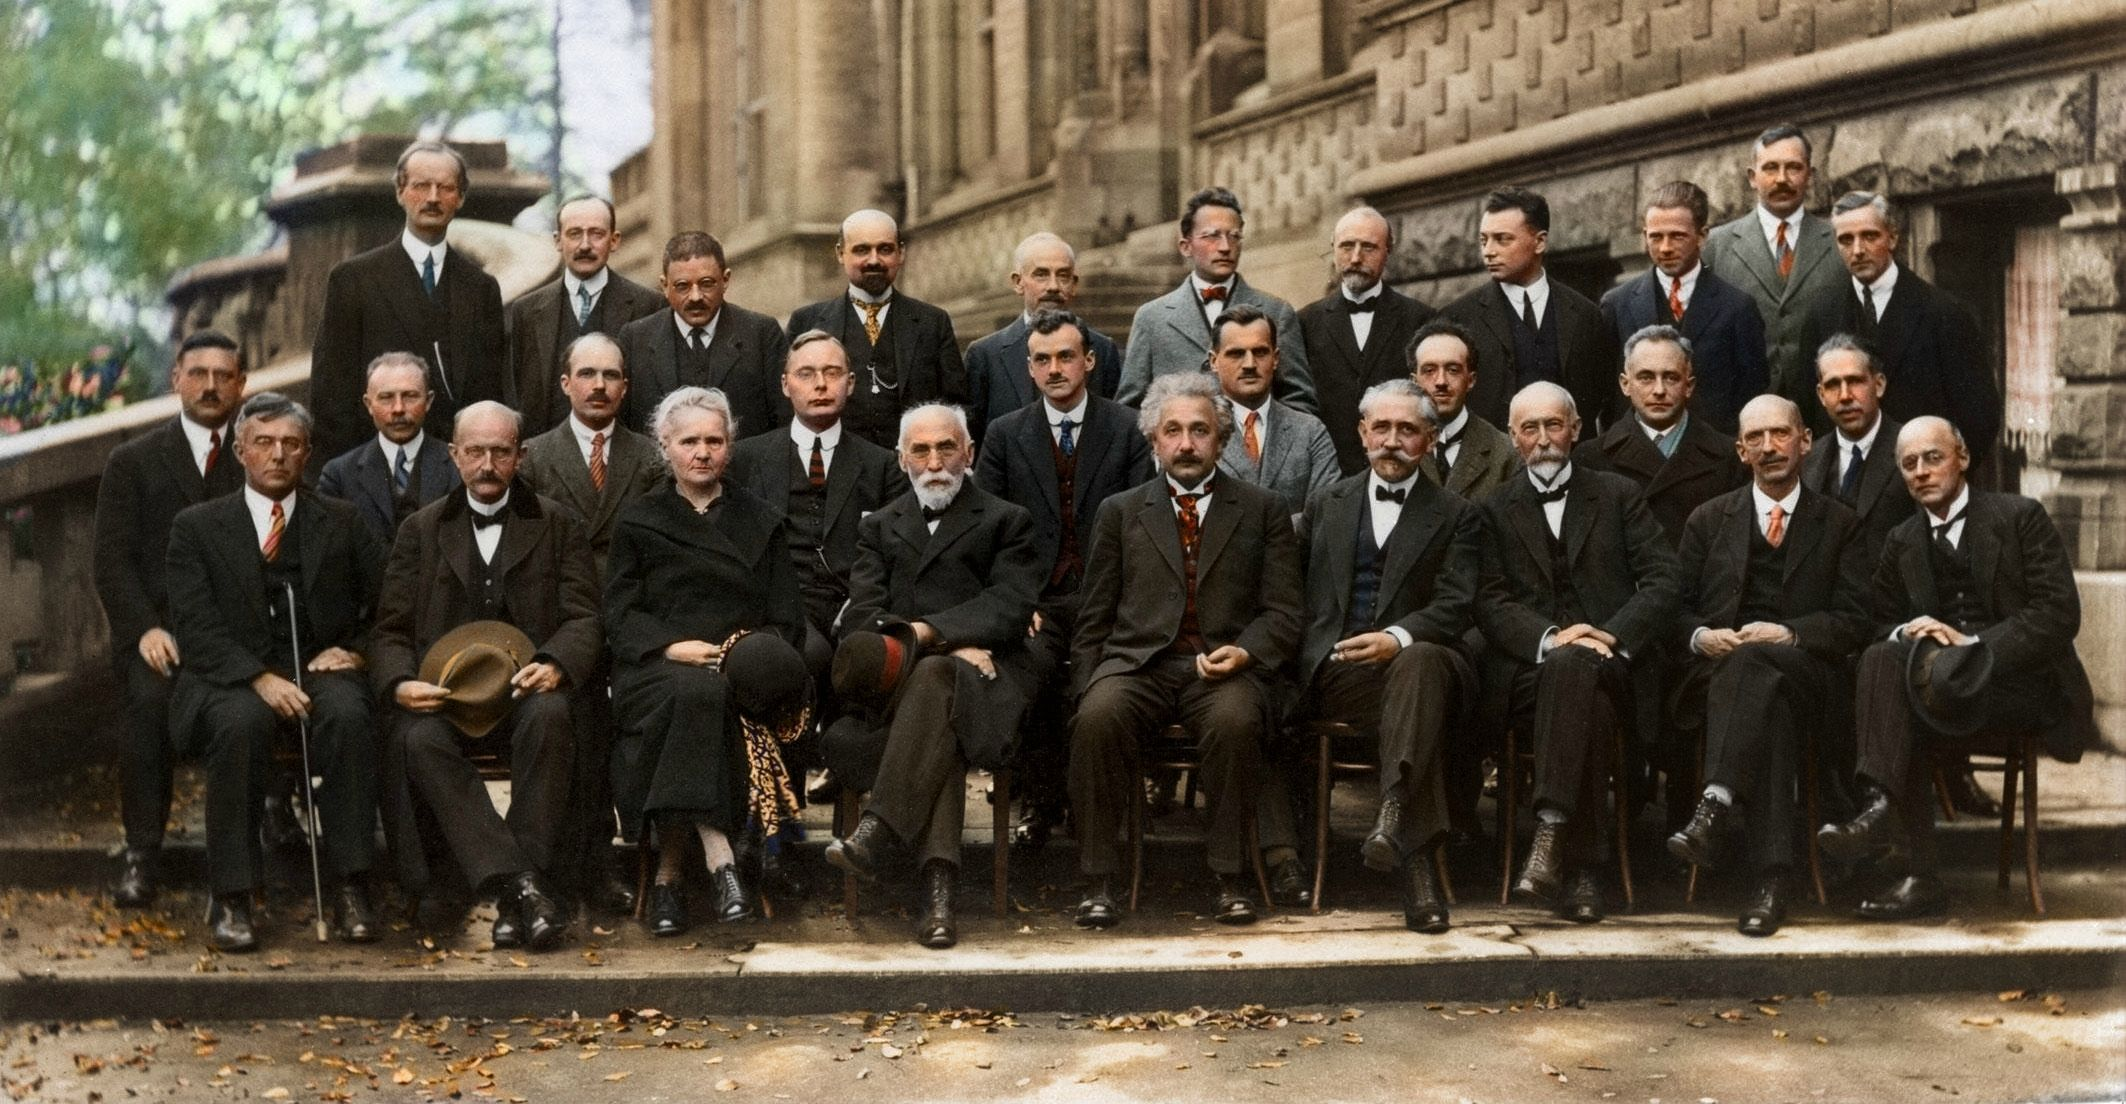
\includegraphics[height=0.57\textwidth,width=1.1\textwidth,viewport=0 0 2150 1050,clip]{Figures/Solvay_Conference-5-fine.jpg}
\vspace{-14.5pt}
\hspace*{-15.5pt}
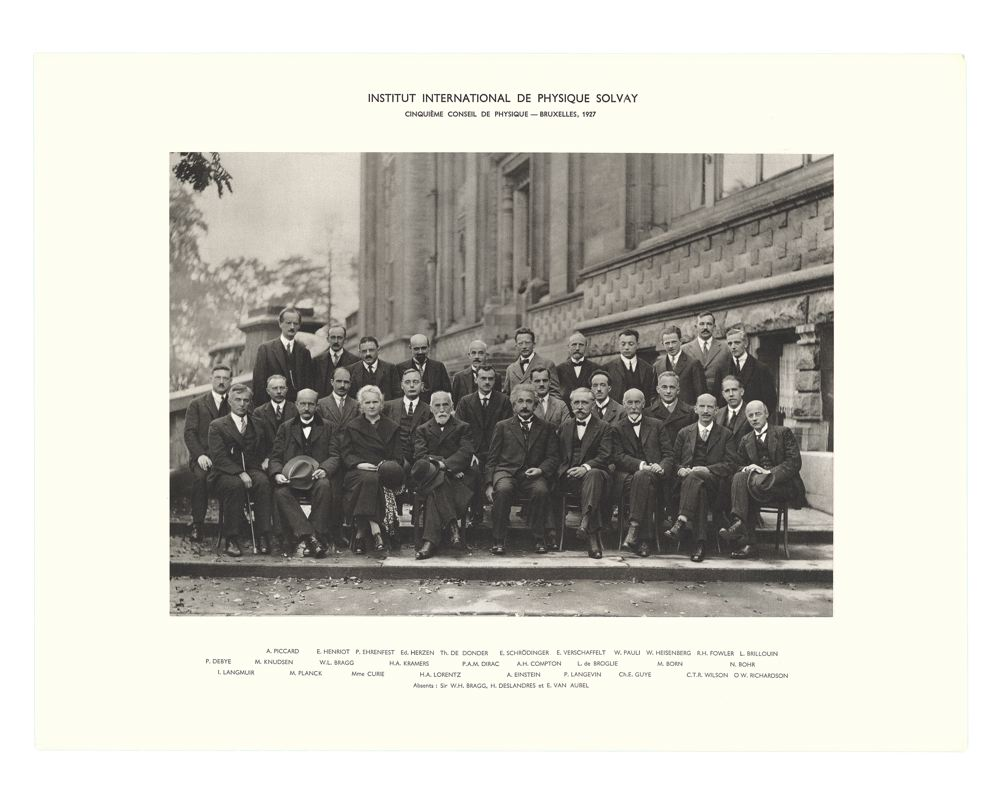
\includegraphics[height=0.50\textwidth,width=0.70\textwidth,viewport=150 105 850 710,clip]{Figures/Solvay_Conference-5.jpg}
\caption{\fontsize{7.5pt}{6.2pt}\selectfont{\textrm{The Fifth Solvay International Conference, Brussels, Belgium, Oct. 1927}}}
\label{Solvay Conference-5-fine}
\end{figure}
\vspace{-11.5pt}
\fontsize{4.1pt}{3.9pt}\selectfont{\textrm{\textcolor{blue}{前排左起}:~I.Langmuir(\textcolor{blue}{朗缪尔}) M.Planck(\textcolor{blue}{普朗克}) Marie Curie(\textcolor{blue}{居里夫人}) H.Lorentz(\textcolor{blue}{洛仑兹}) A.Einstein(\textcolor{blue}{爱因斯坦}) P.Langevin(\textcolor{blue}{朗之万}) Ch.E.Guye(\textcolor{blue}{古伊}) C.T.R.Wilson(\textcolor{blue}{威尔逊}) O.W.Richardson(\textcolor{blue}{理查森})\\
\textcolor{blue}{中排左起}:~P.Debye(\textcolor{blue}{德拜}) M.Knudsen(\textcolor{blue}{克努森}) W.L.Bragg(\textcolor{blue}{布拉格}) H.A.Kramers(\textcolor{blue}{克莱默}) P.A.M.Dirac(\textcolor{blue}{狄拉克}) A.H.Compton(\textcolor{blue}{康普顿}) L.de Broglie(\textcolor{blue}{德布罗意}) M.Born(\textcolor{blue}{玻恩}) N.Bohr(\textcolor{blue}{玻尔})\\
\textcolor{blue}{后排左起}:~A.Piccard(\textcolor{blue}{皮卡尔德}) E.Henriot(\textcolor{blue}{亨利厄特}) P.Ehrenfest(\textcolor{blue}{埃伦费斯特}) Ed.Herzen(\textcolor{blue}{赫尔岑}) Th.de Donder(\textcolor{blue}{德唐德}) E.Schr\"odinger(\textcolor{blue}{薛定谔}) E.Verschaffelt(\textcolor{blue}{费尔夏费尔特}) W.Pauli(\textcolor{blue}{泡利}) W.Heisenberg(\textcolor{blue}{海森堡}) R.H.Fowler(\textcolor{blue}{富勒}) L.Brillouin(\textcolor{blue}{布里渊})}}
}
%------------------------------------------------------------------------Reference----------------------------------------------------------------------------------------------
\frame
{
	\frametitle{量子力学基本假设(\textcolor{red}{公理体系})}
	\begin{itemize}
		\item 全同粒子假设\\
			\textcolor{blue}{全同粒子组成的体系中,两个全同粒子相互调换不改变体系的状态}\\ 
			全同粒子是指\textcolor{red}{内禀性质完全相同的一类微观粒子}:\\例如,所有的电子是全同粒子 
		\item 波函数假设\\
			\textcolor{blue}{微观体系的运动状态可由波函数$\Psi$完全描述,波函数包含体系的所有性质}\\
			波函数$\Psi$一般要求满足\textcolor{red}{连续}、\textcolor{red}{有限}和\textcolor{red}{单值}三个条件
		\item 态叠加原理\\
			如果$\Psi_1$是体系的一个本征态,对应的本征值为$A_1$,$\Psi_2$也是体系的一个本征态,对应的本征值为$A_2$,则\textcolor{blue}{$$\Psi=C_1\Psi_1+C_2\Psi_2$$}\textcolor{red}{也是体系一个可能的存在状态}
	\end{itemize}
}

\frame
{
	\frametitle{Schr\"odinger's cat}
\begin{figure}[h!]
\centering
\vspace{-10.5pt}
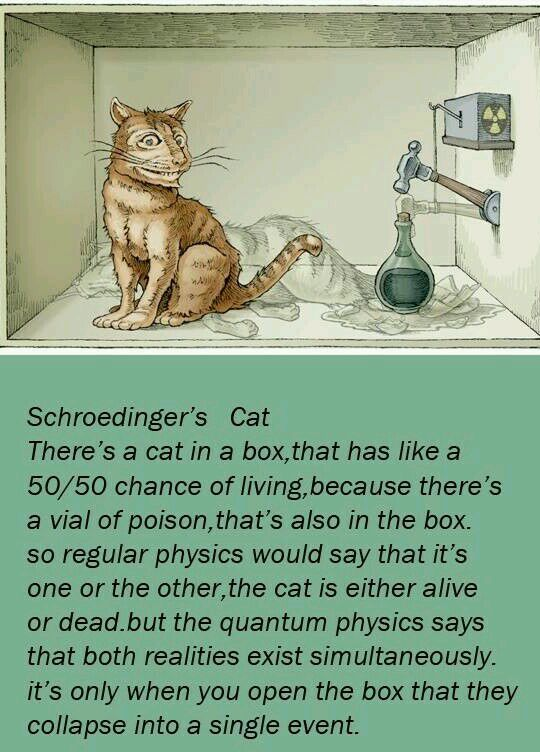
\includegraphics[height=0.70\textwidth,width=0.7\textwidth,viewport=0 0 760 750,clip]{Figures/Schrodinger-cat.jpg}
%\caption{\textrm{ABINIT}的Si.in}
\label{Schrodinger-cat}
\end{figure}
}

\frame
{
	\frametitle{量子力学基本假设(续)}
	\begin{itemize}
		\item 力学量算符假设\\
			\textcolor{blue}{经典力学中的物理量对应到量子力学中,要用线性\textrm{Hermite~}算符表示}(\textcolor{red}{\textrm{Hermite~}算符的本征函数构成完备空间})\\
			如动量算符 
			$$\hat{\mathbf{p}}=-\mathrm{i}\hbar\nabla$$
			位置算符$$\hat{\mathbf r}=r$$
			力学量算符之间有确定的对易关系(量子条件)
			$$[\hat{\mathbf F},\hat{\mathbf G}]=\hat{\mathbf F}\hat{\mathbf G}-\hat{\mathbf G}\hat{\mathbf F}$$ 
			
		\item 微观体系的运动状态\textcolor{blue}{波函数随时间变化的规律}:\\\textcolor{red}{遵从\textrm{Schr\"odinger}方程}
			$$\mathrm{i}\hbar\dfrac{\mathrm{d}}{\mathrm{d}t}|\Psi\rangle=\hat{\mathbf H}|\Psi\rangle$$
	\end{itemize}
}

\frame
{
	\frametitle{\rm{Paul Dirac's Commandments}}
	\textrm{\textcolor{purple}{The fundamental laws necessary for the mathematical treatment of a large part of physics and the whole of chemistry are thus completely known, and the difficulty lies only in the fact that application of these laws leads to equations that are too complex to be solved.}}
}

%\frame
%{
%	\frametitle{量子力学基本假设(续)}
%  \begin{tikzpicture}
%    \coordinate (O) at (0,0);
%    \fill (O) circle (1pt);
%    \draw[dashed] (O) circle (3);
%    \draw[domain=0:2.1*pi,samples=400,line width=1pt]
%      plot ({deg(\x)}:{3+0.5*sin(deg(7.4*\x))});
%  \end{tikzpicture}
%
%  \begin{tikzpicture}
%    \coordinate (O) at (0,0);
%    \fill (O) circle (1pt);
%    \draw[dashed] (O) circle (3);
%    \draw[domain=0:2*pi,samples=400,line width=1pt]
%      plot ({deg(\x)}:{3+0.5*sin(deg(8*\x))});
%
%    \draw (56.25:3.6) --+ (56.25:0.4) (101.25:3.6) --+ (101.25:0.4);
%    \draw[<->] (56.25:3.8) arc (56.25:101.25:3.8);
%    \node at (78.75:4){$\lambda$};
%    \draw[->] (O) -- (50:3);
%  \end{tikzpicture}
%}
%------------------------------------------------------------------------Reference----------------------------------------------------------------------------------------------
%\begin{thebibliography}{99}
%-----------------------------------------------------------------------------------------------------------------------------------------------------------------------%
%\frame
%{
%\frametitle{主要参考文献}
%{\small
%\bibitem{Singh_Book}\textrm{D. J. Singh. \textit{Plane Wave, PseudoPotential and the LAPW method} (Kluwer Academic, Boston,USA, 1994)}					%
%  \nocite{*}																				%
%}
%}
%\end{thebibliography}

%-----------------------------------------------------------Beamer下不建议使用bib,因为涉及分页--------------------------------------------------------------------------%
\frame[allowframebreaks]
{
\frametitle{主要参考文献}
{\tiny\textrm{
%\phantomsection\addcontentsline{toc}{section}{Bibliography}	 %直接调用\addcontentsline命令可能导致超链指向不准确,一般需要在之前调用一次\phantomsection命令加以修正	%
%\phantomsection\addcontentsline{toc}{section}{主要参考文献}	 %直接调用\addcontentsline命令可能导致超链指向不准确,一般需要在之前调用一次\phantomsection命令加以修正	%
\bibliography{../ref/Myref}																			%
\bibliographystyle{../ref/mybib}																		%
}}
%\nocite{*}																				%
}
%------------------------------------------------------------------------------------------------------------------------------------------------------------------------------%

%-------------------------------------------------------------------------Thanks------------------------------------------------------------------------------------------------
%\section{致谢}
%\frame
%{
%\frametitle{致$\quad$谢}
%\begin{itemize}
%    \setlength{\itemsep}{20pt}
%  \item 感谢本团队高兴誉、吴泉生、宋红州等各位老师参与的讨论
%  \item 感谢莫所长、宋主任以及软件中心各位老师和同事
%  \item 感谢王崇愚先生的帮助
%\end{itemize}
%}

\logo{}									%不显示logo
\frame
{
\vskip 60 pt
%\hskip 10pt \textcolor{blue}{\Huge 感谢答辩委员会各位老师\,\textrm{!}}\\
\vskip 35 pt
\hskip 60pt \textcolor{blue}{\Huge 谢谢大家\:!}
%\vskip 15 pt
%\hskip 40pt \textcolor{blue}{\Huge \textrm{for your attention\:!}}
}

%\frame
%{
%\begin{figure}[h!]
%\centering
%\animategraphics[autoplay, loop, height=2.1in]{1}{Figures/Prof_Liu-}{06}{11}
%\label{Prof_Liu}
%\end{figure}
%}
%
%-------------------------------------------------------------------------------------------------------------------------------------------------------------------------------

\clearpage
%\end{CJK*}
\end{document}
